\section{Background}

Possessing the ability of flight and minimising effort and casualties has always been desirable for the utility flight can provide.
The first unmanned aircrafts can be dated back to 1849, where Austria seemingly had utilised unmanned air balloons with stuffed explosives to attack Venice. \cite{Vyas2020}
Ever since an unmanned aircraft vehicle (UAV), is one that is flown by technological means or as a pre-programmed flight without pilot control, as defined by the ECAA Transport Agency \cite{Droner}, nowadays called drones, have risen in popularity.


Because of this, UAVs come in a wide range of sizes and weights.
UAVs often include multirotor, radio-controlled miniature helicopters, and aeroplanes \cite{Ann2012}.
As a result, there are several methods to categorize drones. The performance parameters of UAVs, such as weight, wingspan, wing load, flight range, maximum flying altitude, speed, and production cost, are typically used to categorize them \cite{Hassanalian2017}.
According to how the lift is produced, drones may also be divided into fixed-wing and rotating-wing types.
According to the drone code category, the European Aviation Safety Agency (EASA) categorizes unmanned aircraft by weight.
The EASA regulations for open categories, or drones without an EASA class designation, are summarized succinctly and simply in Figure~\ref{fig:Table} \cite{Euasa}.

Self-built drones weighing up to 250 g, as described in Figure~\ref{fig:Table}, may be used without registration if the drone is a toy or the drone is not equipped with a camera, the remaining drones must be registered, and the pilot must pass examinations \cite{Euasa}. In this paper, self-built rotary drones with four wings or propellers are the objective, making weight-based classification suitable.

\begin{figure}[H]
    \centering
    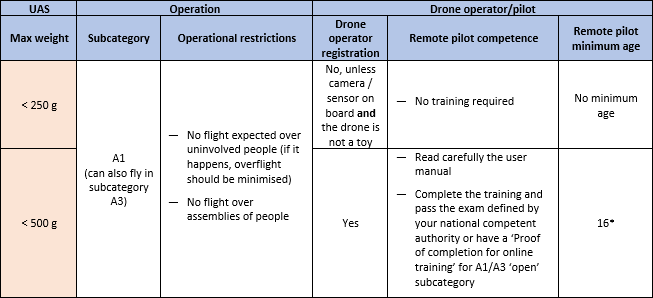
\includegraphics[scale = 0.9]{pictures/classification.PNG}
    \caption{Classification and restrictions for non-EASA class drones \cite{Euasa}}
    \label{fig:Table}
\end{figure}


When it comes to the state-of-the-art project, PULP-DroNet is a deep learning-powered visual navigation engine that enables autonomous navigation of a pocket-size quadrotor in a previously unseen environment. Thanks to PULP-DroNet the nano-drone can explore the environment, avoiding collisions also with dynamic obstacles, in complete autonomy -- no human operator, no ad-hoc external signals, and no remote laptop! This means that all the complex computations are done directly aboard the vehicle and very fast. The visual navigation engine is composed of both a software and a hardware part. \cite{Niculescu2021}

When it comes to the future, the simulated pollination of agricultural plants by means of nano copter can provide collecting and delivering pollen in the mode of automatic control. A design of nano copter for pollination can be made on the basis of innovative modification of existing model by its reprogramming with regard to its flight controller that is to be fully adapted to computer interface. The robotic system is offered specially for artificial pollination in conditions of greenhouses and minor agricultural enterprises. \cite{Abutalipov2016}